\subsection{Test Journal: Preliminary VTS model frequency sweep} \label{app:tj_00}

\textbf{Executed by: Martin Therkildsen} \\
\textbf{Date: 05/10/2022}

\subsubsection{Objective}
This test aims to document the behaviour of the floating Vestas Turbine Simulator (VTS) model in the first semi-successful preliminary frequency sweep test. It is desired to get an understanding of how the floating turbine is operating when the different rotor frequencies are induced and how these frequencies translate into the structure of the turbine.

\subsubsection{Background}
A Vestas matlab tool called SysIdFrqSweep is able to generate Design Load Cases (DLCs) which make a variable such as the rotor speed include a constant frequency as to analyse how such a frequency translates to the rest of the system mainly of interest the y-direction foundation translation and tower pitch angle. Essentially it should be possible to make a bode plot when enough simulations are run at enough frequencies. This could be used to tune the linear model to match the VTS model as closely as possible. As such bode plots would also be made for the linear model and compared.

\subsubsection{Test subject}
The test subject is a specific floating turbine setup which is simulated with VTS. The turbine is a V164 8MW on a floating semi-submersible platform.

\subsubsection{Equipment/Software used and test setup}
The software used for this test is:
\begin{itemize}
	\item \textbf{fat1}: Vestas' simulation prepping software
	\item \textbf{VTS}: Vestas' turbine simulator software
	\item \textbf{OrcaFlex}: A floating foundation simulation tool which communicates with VTS to make floating simulations
	\item \textbf{Matlab}: To make fast fourier transforms fft of the data and to plot the data in figures
	\item \textbf{SysIDFrqSweep matlab tool}: A Vestas matlab tool which generates load cases which are put into the turbine prep file to simulate variables oscillating at chosen frequencies
\end{itemize}


\subsubsection{Test procedure}
SysIdFrqSweep is used to generate in this test to generatoe 10 different frequencies which are to be applied to the rotor speed. These frequencies are merely put on top of the rotational velocity of the turbine rotor. The rotor will still act according to the simulated physical environment. As such when the tower pitches and moves around the rotor speed will still change accordingly.

The generated rotor frequencies which are generated  are: $0.01, 0.02 ... 0.1$.

The generated prep file is run through fat1 which prepares (preps) the file such that VTS and OrcaFlex can run the simulation. The simulation is set to run a 1800 second simulation.

When the simulation is finished several types of files are output which can be used to analyze what happened during the simulation. ".int" files are sensor file which are virtual sensor readings and products of treated sensors readings. Data from these files are the ones who are plotted in Matlab.

Errors occurred on frequencies 0.01 and 0.03 and as such these could not be plotted in this test. This leaves eight different frequencies.

In Matlab a script made by me extracts the data from the .int files by using a LaC matlab tool. A subset of data is made by fourier transforming all the data such that ffts can also be plotted. The data is then plotted in figures as results.


\subsubsection{Results and Comments}
Since there are 8 different frequencies the data is plotted in sets of four frequencies. Not all all plots of all frequencies are included. 

The first two plots are plots of the free wind speed, blade pitch angle 1, rotor angular velocity and generator torques for the two sets of four frequencies respectively. Frequencies 0.02 to 0.06 are seen in \cref{fig:tjj0_f02to06VfreeToMgen} and frequencies 0.07 to 0.1 are seen in \cref{fig:tjj0_f07to1VfreeToMgen}. The time is restricted to a 100 second window. It is seen that the wind speed is set unrealistically at a constant wind speed such that this disturbance would not interfere with the observations of the system frequencies. Only one blade pitch is plotted since it is deemed redundant to plot all pitch angles as they will all have the same angle at only slightly different amplitudes and slightly different phases. When observing the angular velocities it becomes evident that it is not a trivial task to read out the frequencies added on top of the rotor angular velocity in the timeseries. When observing the rotor angular velocity fft plots in \cref{fig:tjj0_f02to06OmegaFFT} and \cref{fig:tjj0_f07to1_OmegaFFT} the frequencies are apparent as pins at each of the respective frequencies. The frequency content observed at around 0.034 Hz is the natural frequency of the tower-foundation structure in the water.

It is widely evident that the turbine is pitching and translating in the water, resulting in great oscillations in the whole turbine. When looking at the plot of the tower translations and pitch angles in \cref{fig:tjj0_f07to1_xPosToPitchAng} it is obvious that the oscillations are occurring due to the structure movement. An fft of the roll and pitch angles are seen in \cref{fig:tjj0_f07to1_RollPitchAngFFT}.
\begin{figure}[h]
	\centering
	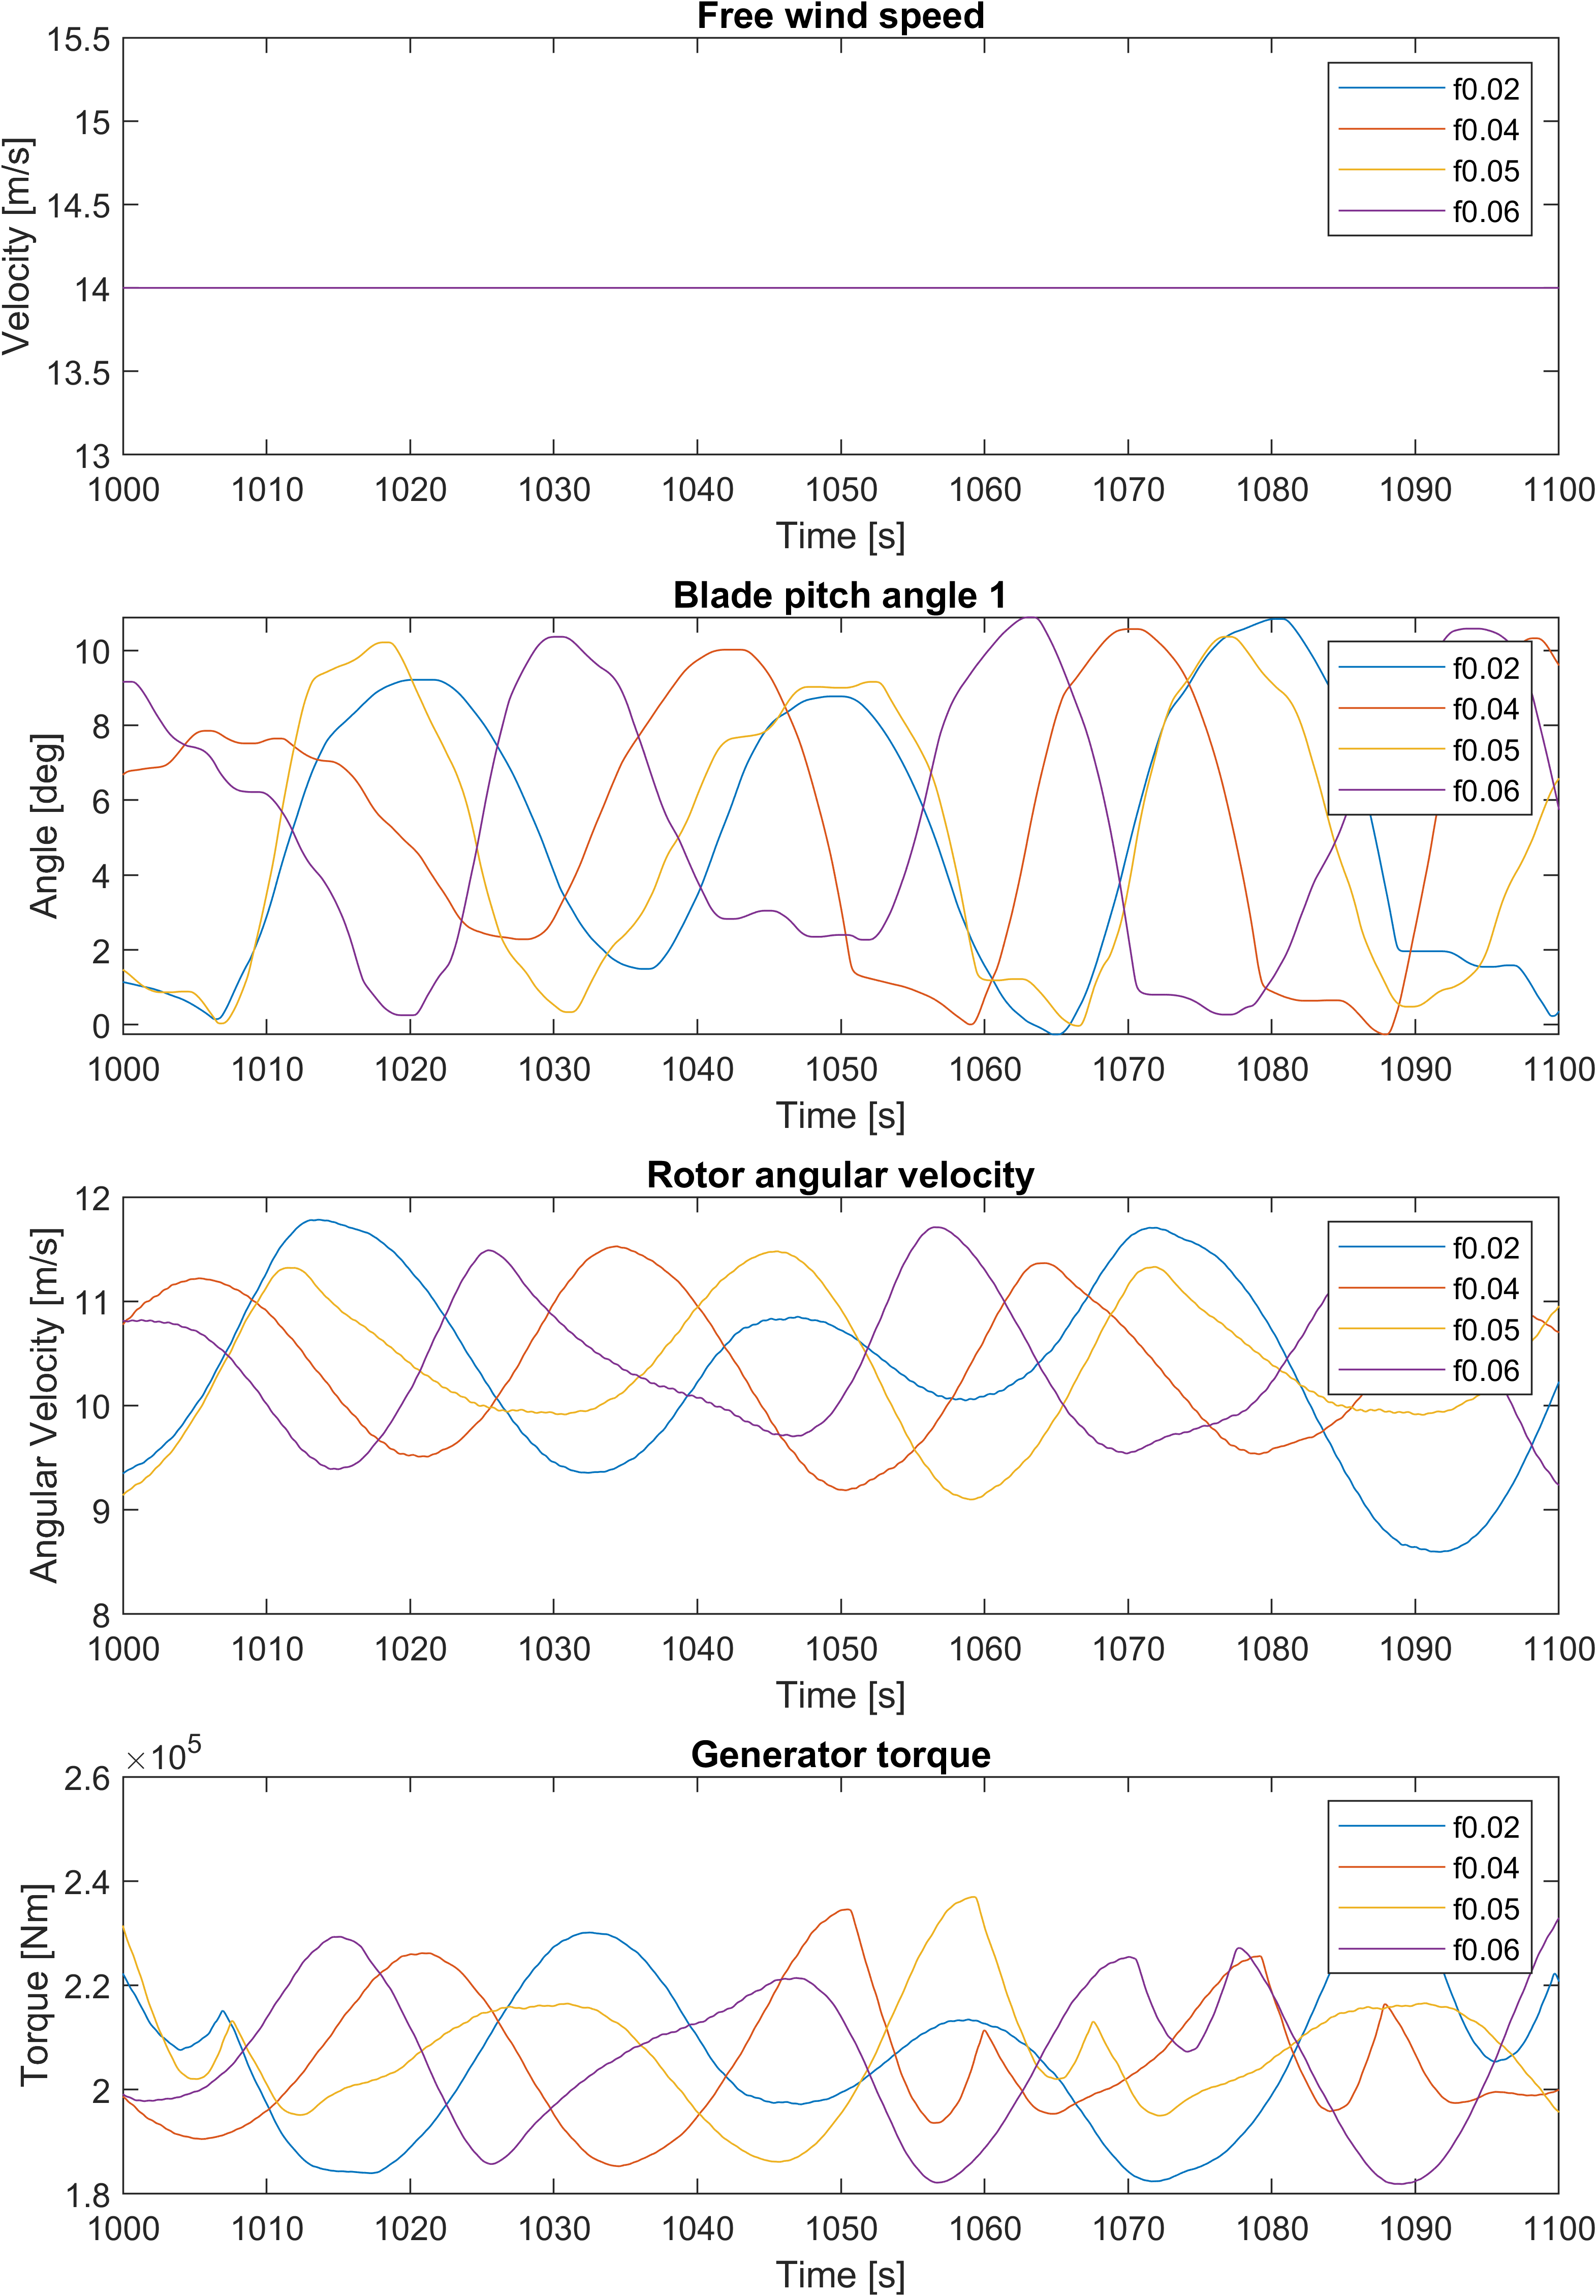
\includegraphics[width=0.8\linewidth]{Graphics/TestResults/tj00/tjj0_f02to06VfreeToMgen.png}
	\caption{Plot of Free wind, Blade pitch angle 1, rotor angular velocity and Generator torque for the injected rotor angular velocity frequencies 0.02 Hz, 0.04 Hz, 0.05 Hz and 0.06 Hz. It is difficult to observe the frequencies directly on the angular velocity.}
	\label{fig:tjj0_f02to06VfreeToMgen}
\end{figure}

\begin{figure}[h]
	\centering
	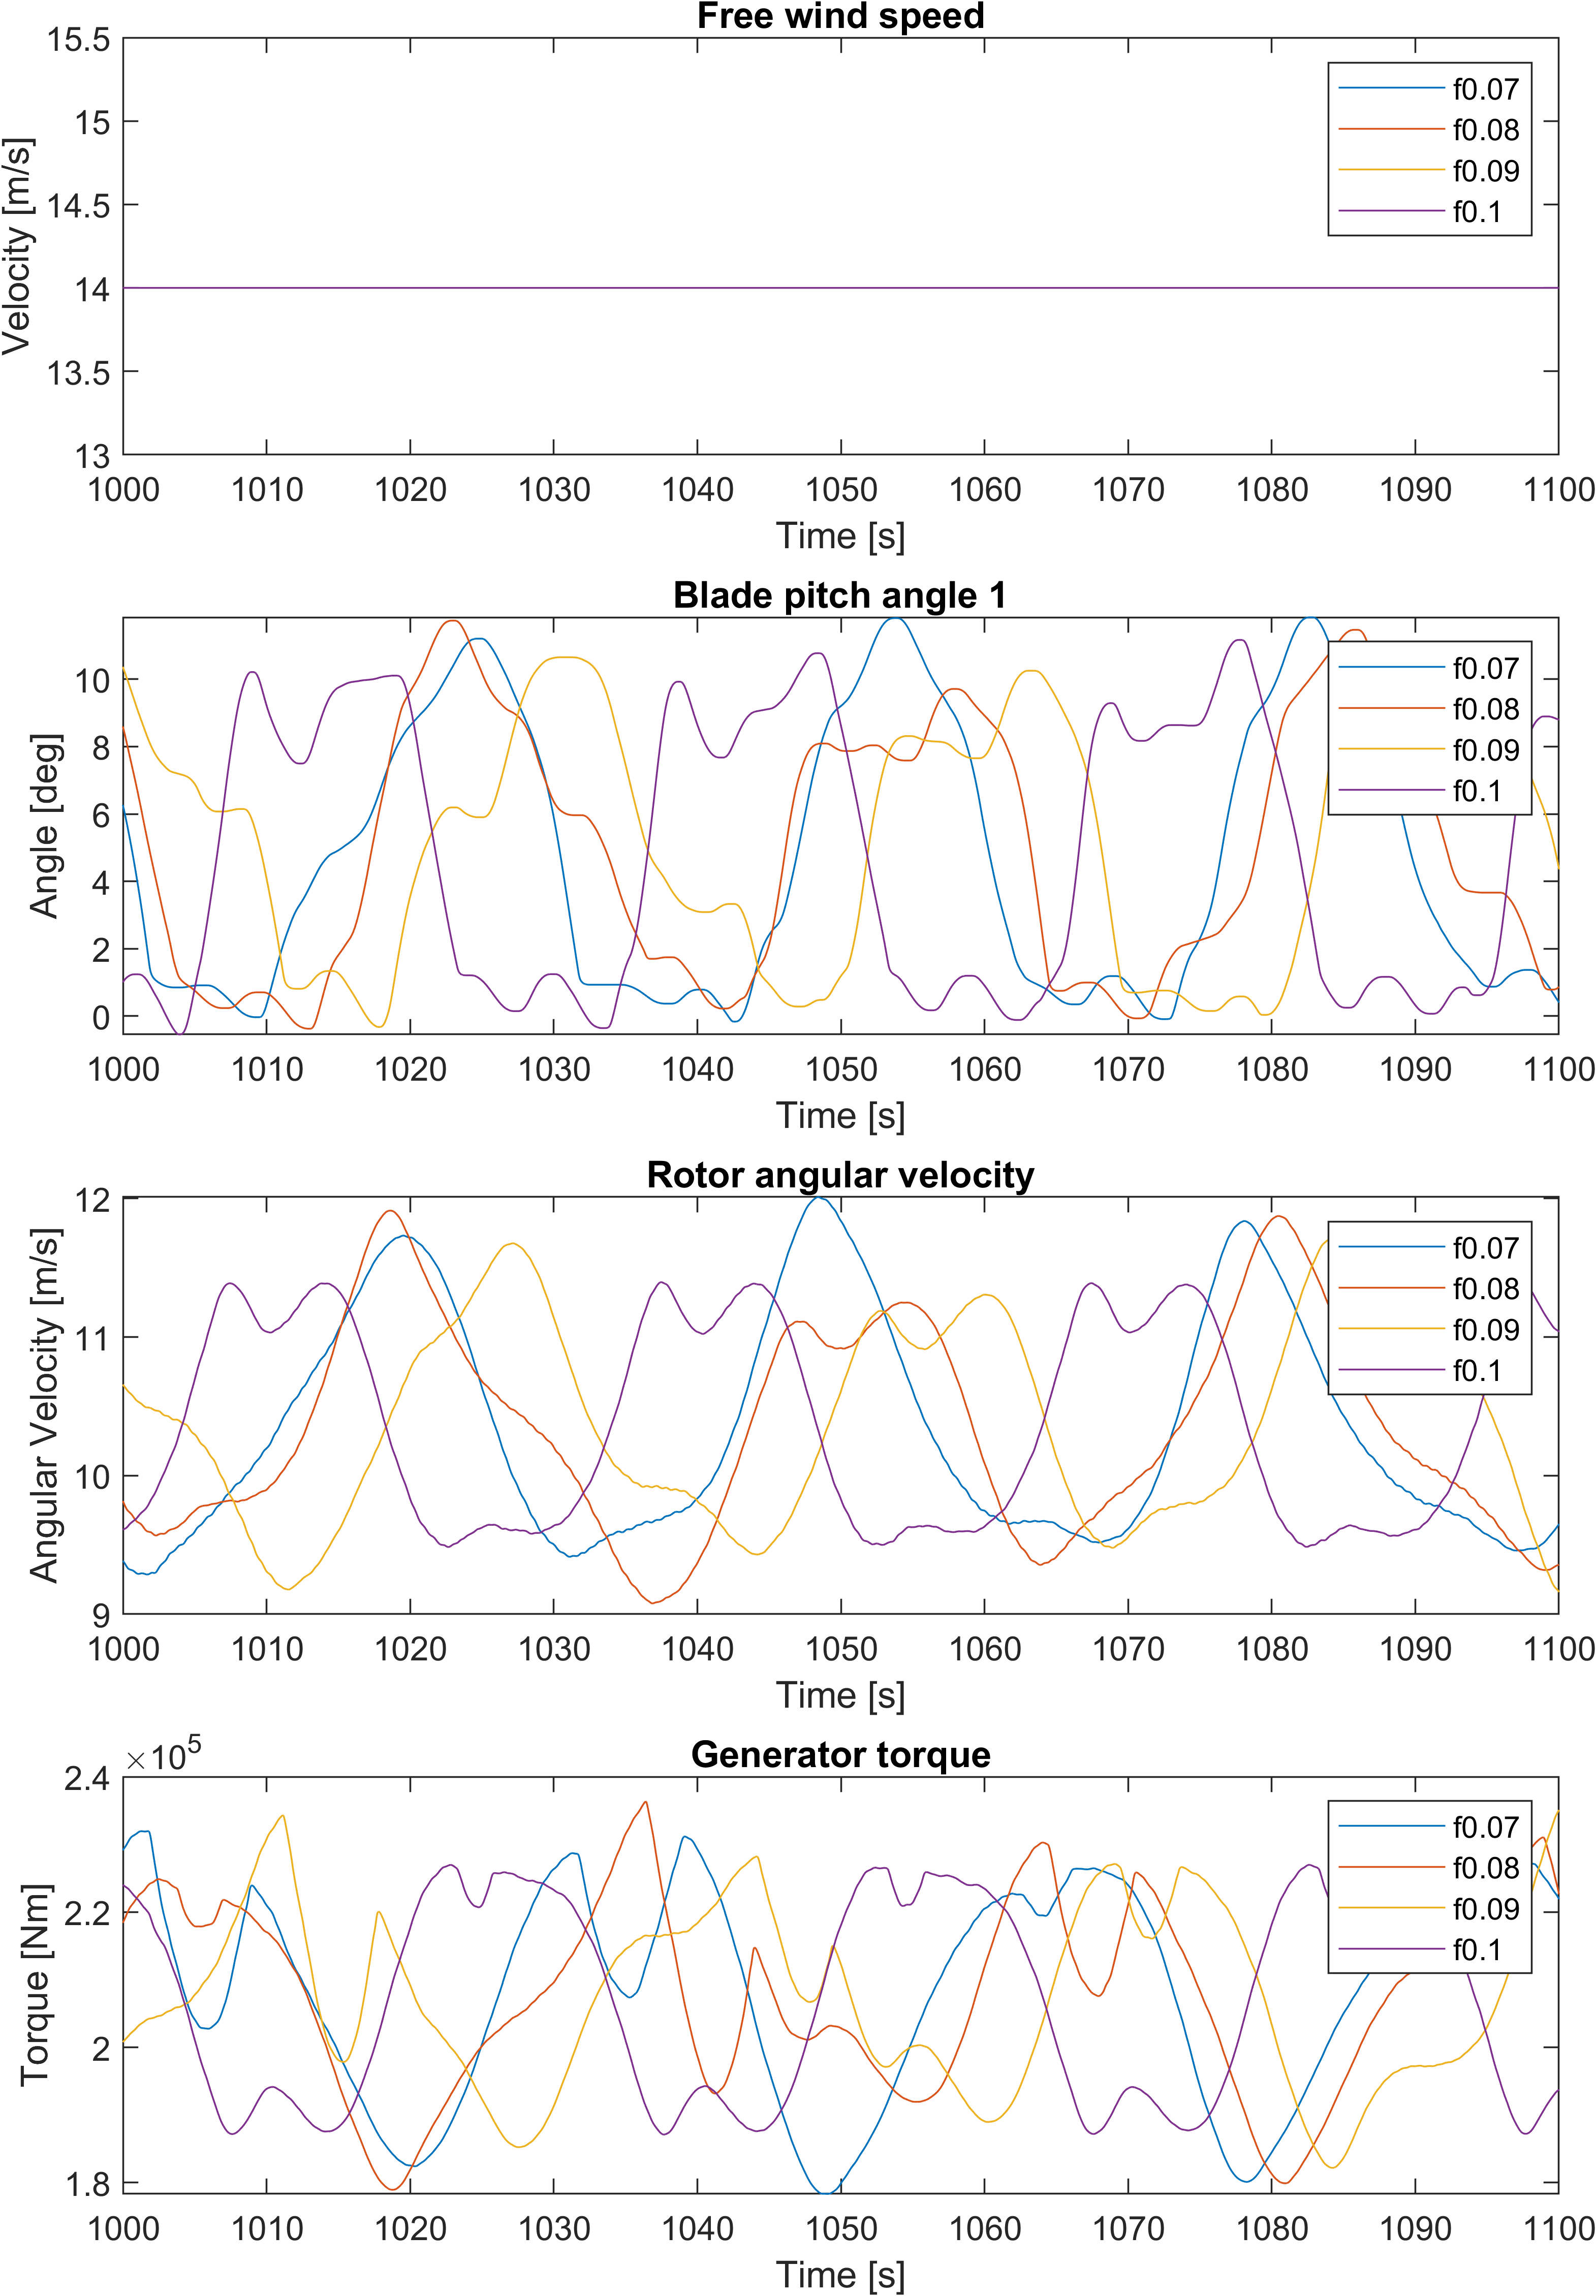
\includegraphics[width=0.8\linewidth]{Graphics/TestResults/tj00/tjj0_f07to1_VfreeToMgen.png}
	\caption{Plot of Free wind, Blade pitch angle 1, rotor angular velocity and Generator torque for the injected rotor angular velocity frequencies 0.07 Hz, 0.08 Hz, 0.09 Hz and 0.1 Hz. It is difficult to observe the frequencies directly on the angular velocity.}
	\label{fig:tjj0_f07to1VfreeToMgen}
\end{figure}

\begin{figure}[h]
	\centering
	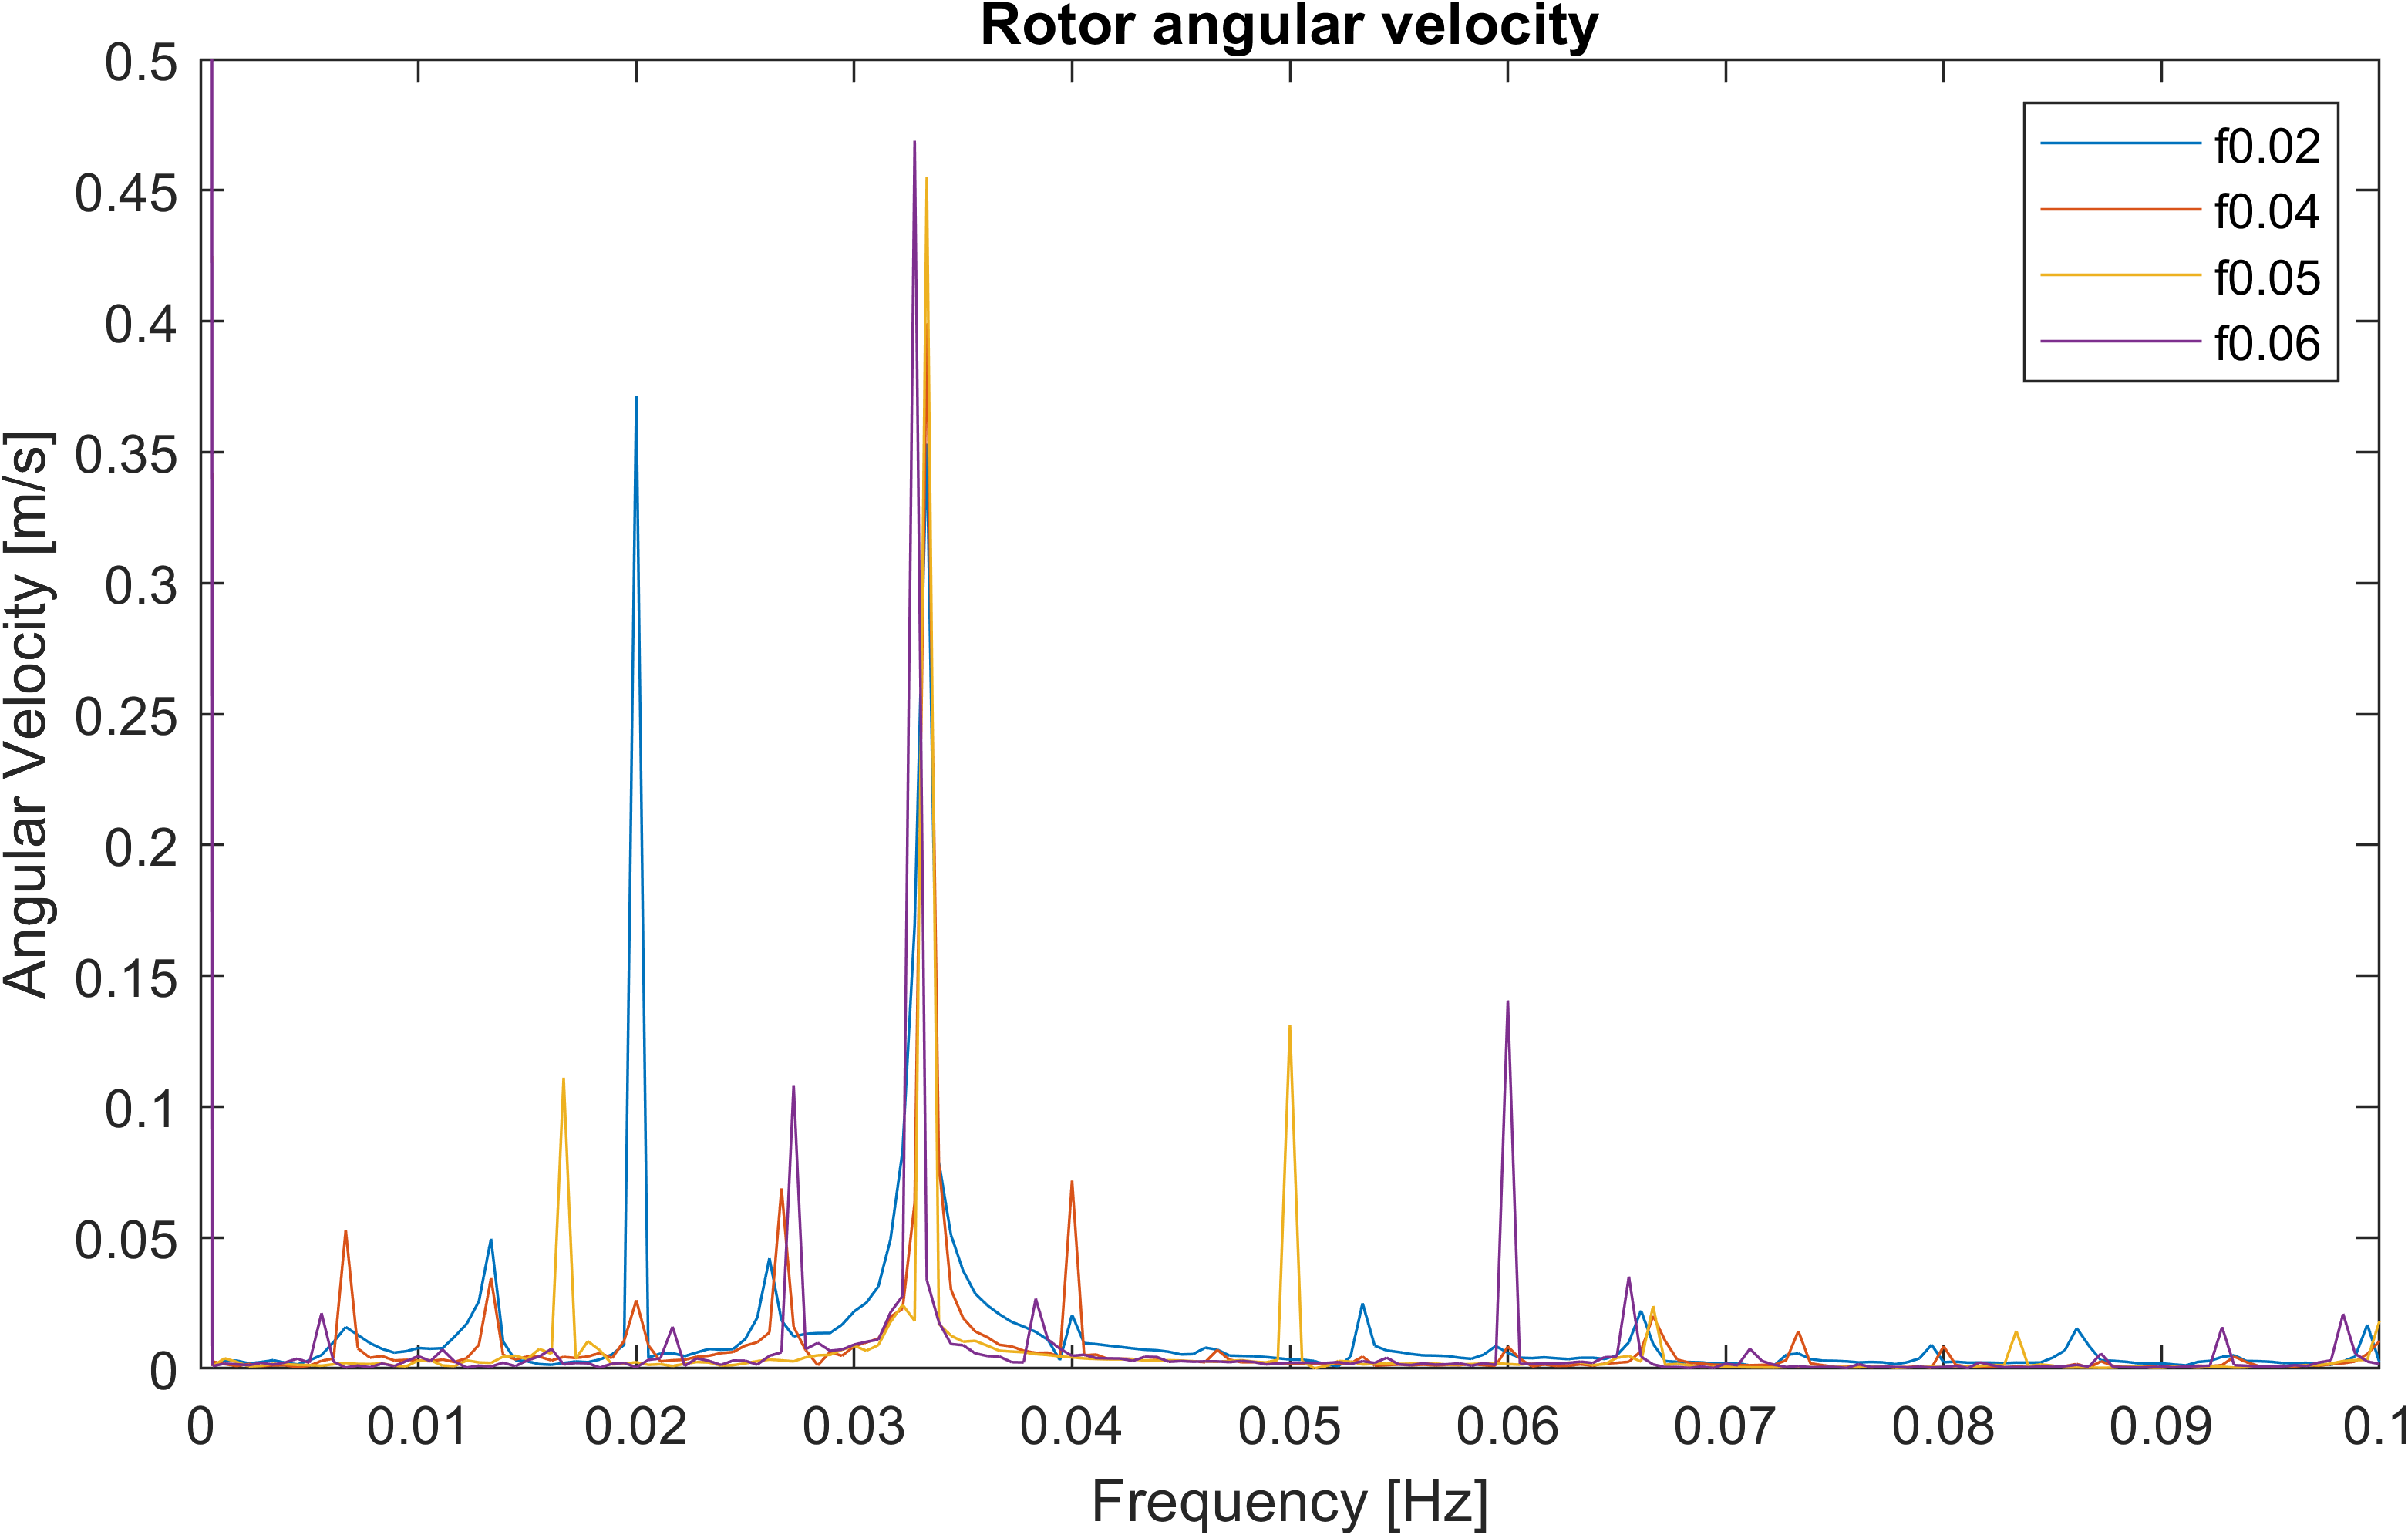
\includegraphics[width=0.8\linewidth]{Graphics/TestResults/tj00/tjj0_f02to06OmegaFFT.png}
	\caption{Plot of FFT of rotor angular velocity for the injected rotor angular velocity frequencies 0.02 Hz, 0.04 Hz, 0.05 Hz and 0.06 Hz. The injected frequencies can be observed as pins at each of the respective frequencies.}
	\label{fig:tjj0_f02to06OmegaFFT}
\end{figure}

\begin{figure}[h]
	\centering
	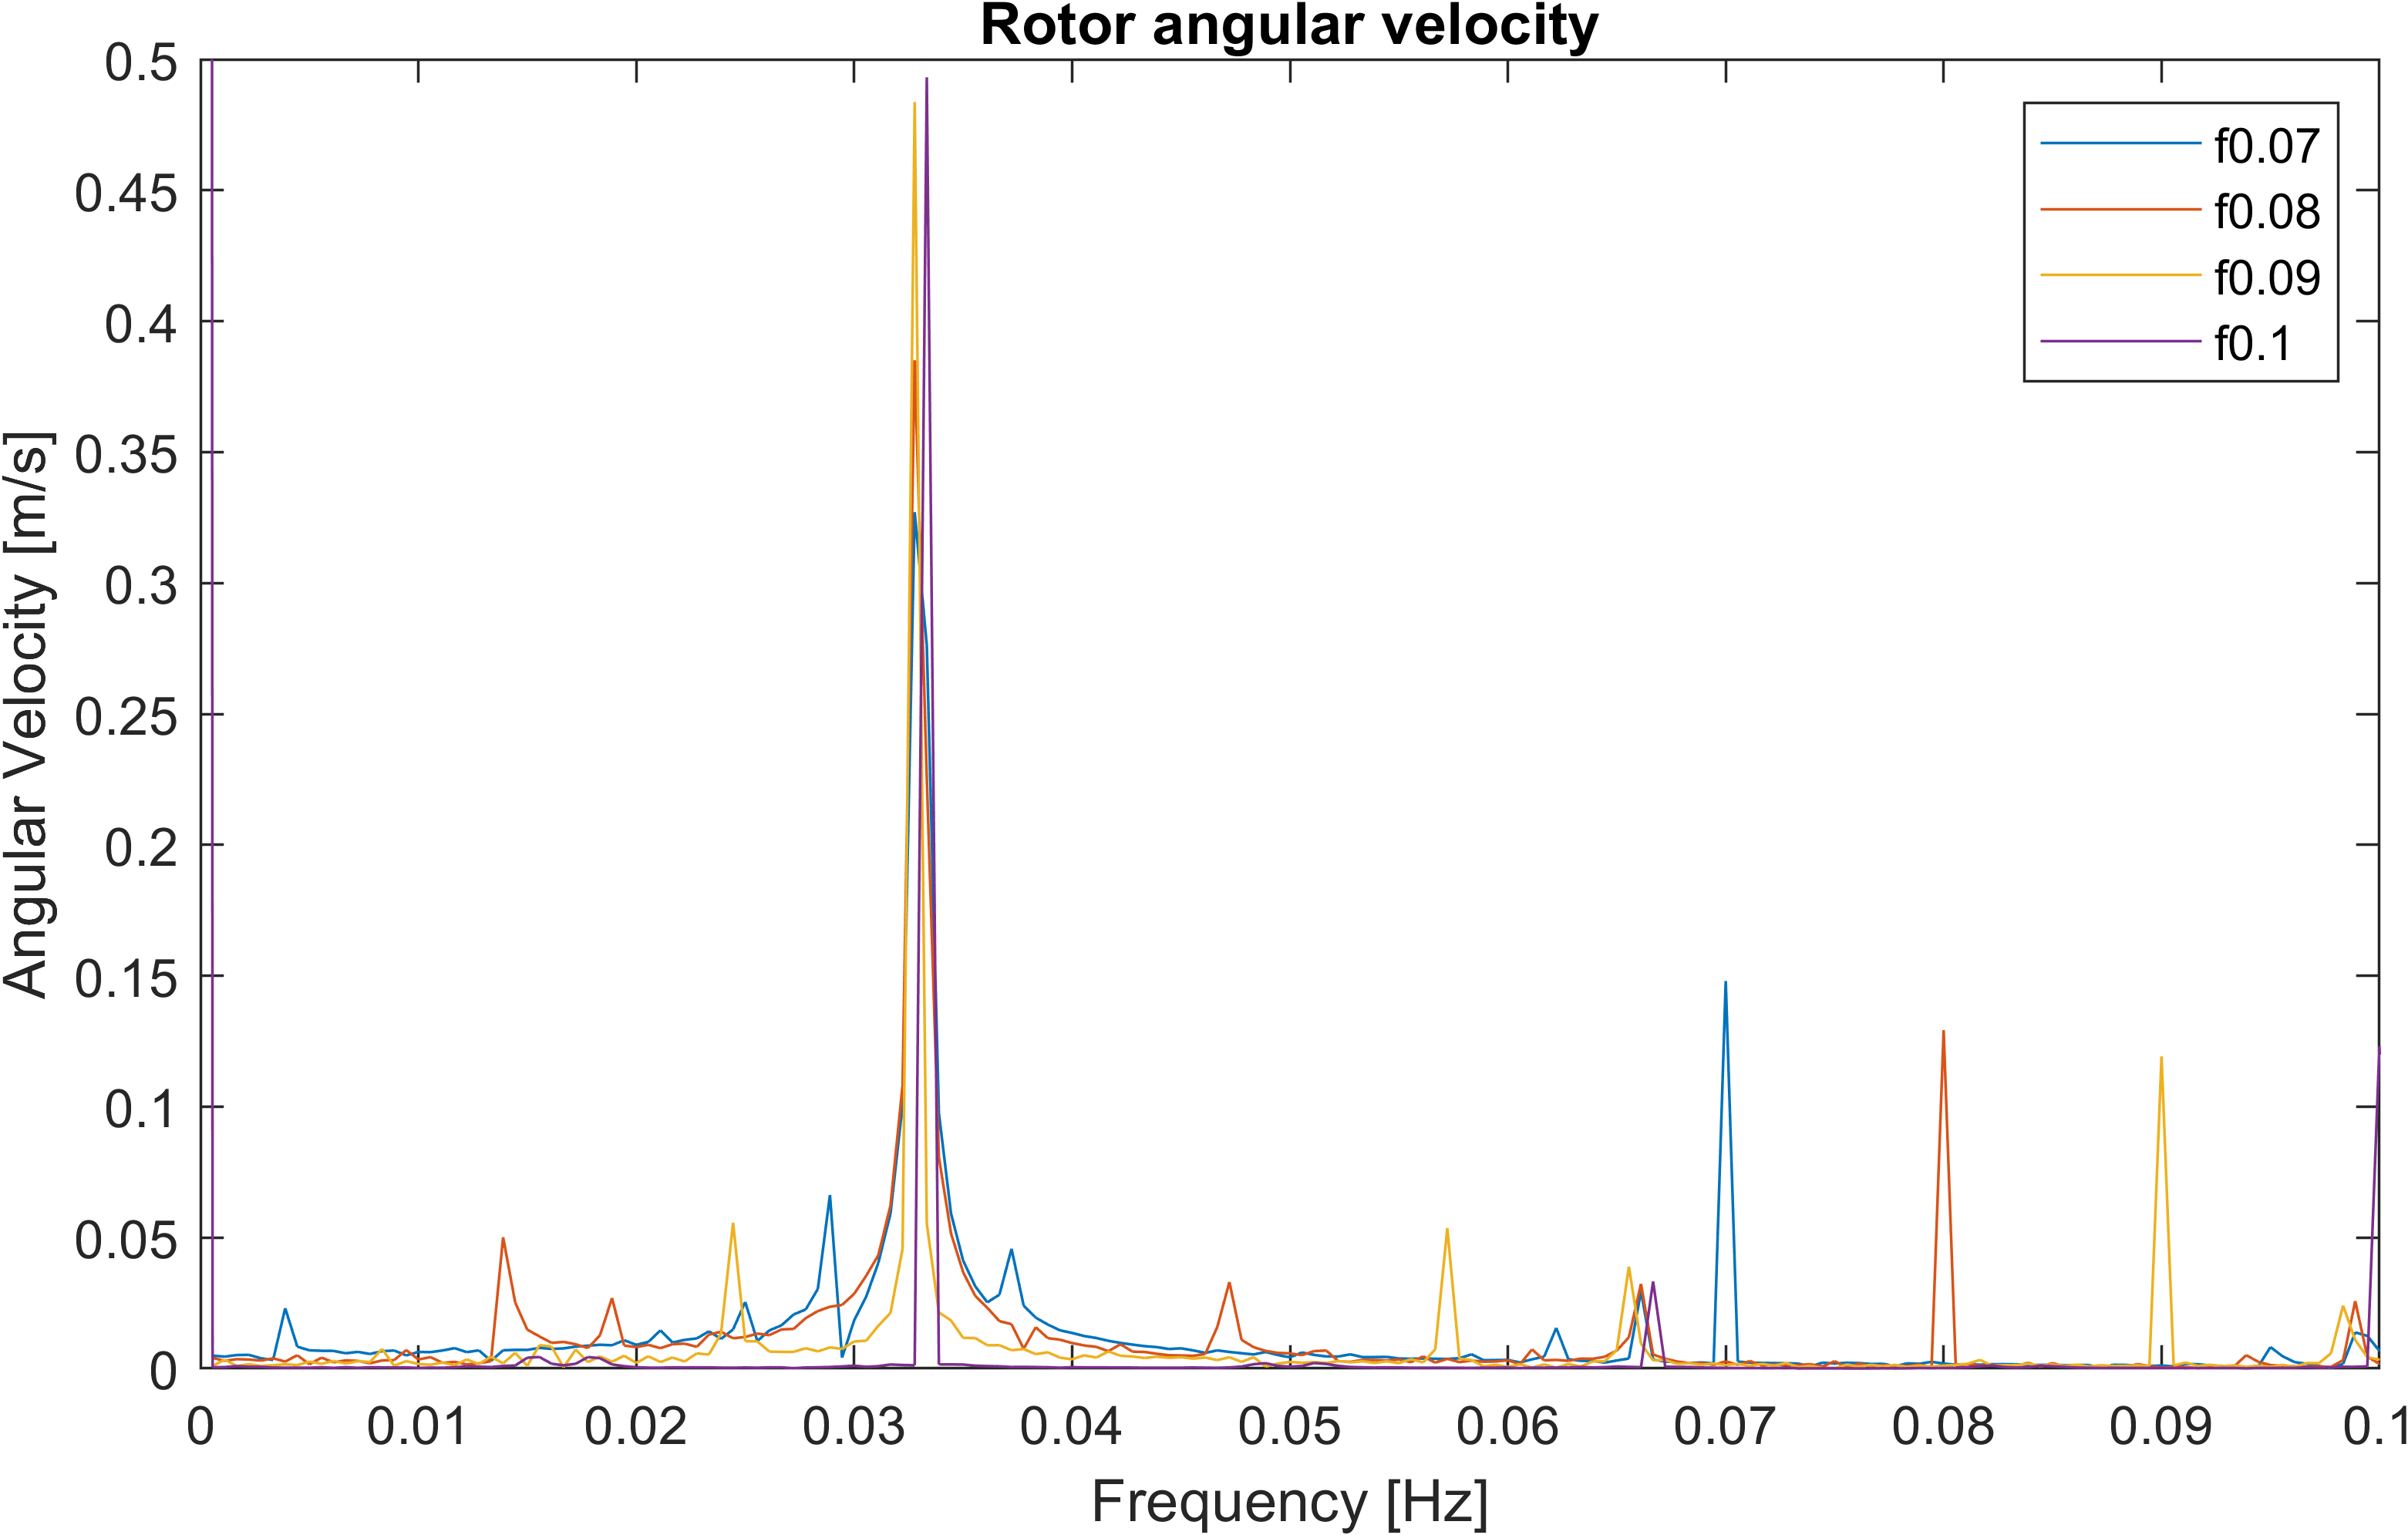
\includegraphics[width=0.8\linewidth]{Graphics/TestResults/tj00/tjj0_f07to1_OmegaFFT.png}
	\caption{Plot of FFT of rotor angular velocity for the injected rotor angular velocity frequencies 0.07 Hz, 0.08 Hz, 0.09 Hz and 0.1 Hz. The injected frequencies can be observed as pins at each of the respective frequencies.}
	\label{fig:tjj0_f07to1_OmegaFFT}
\end{figure}

\begin{figure}[h]
	\centering
	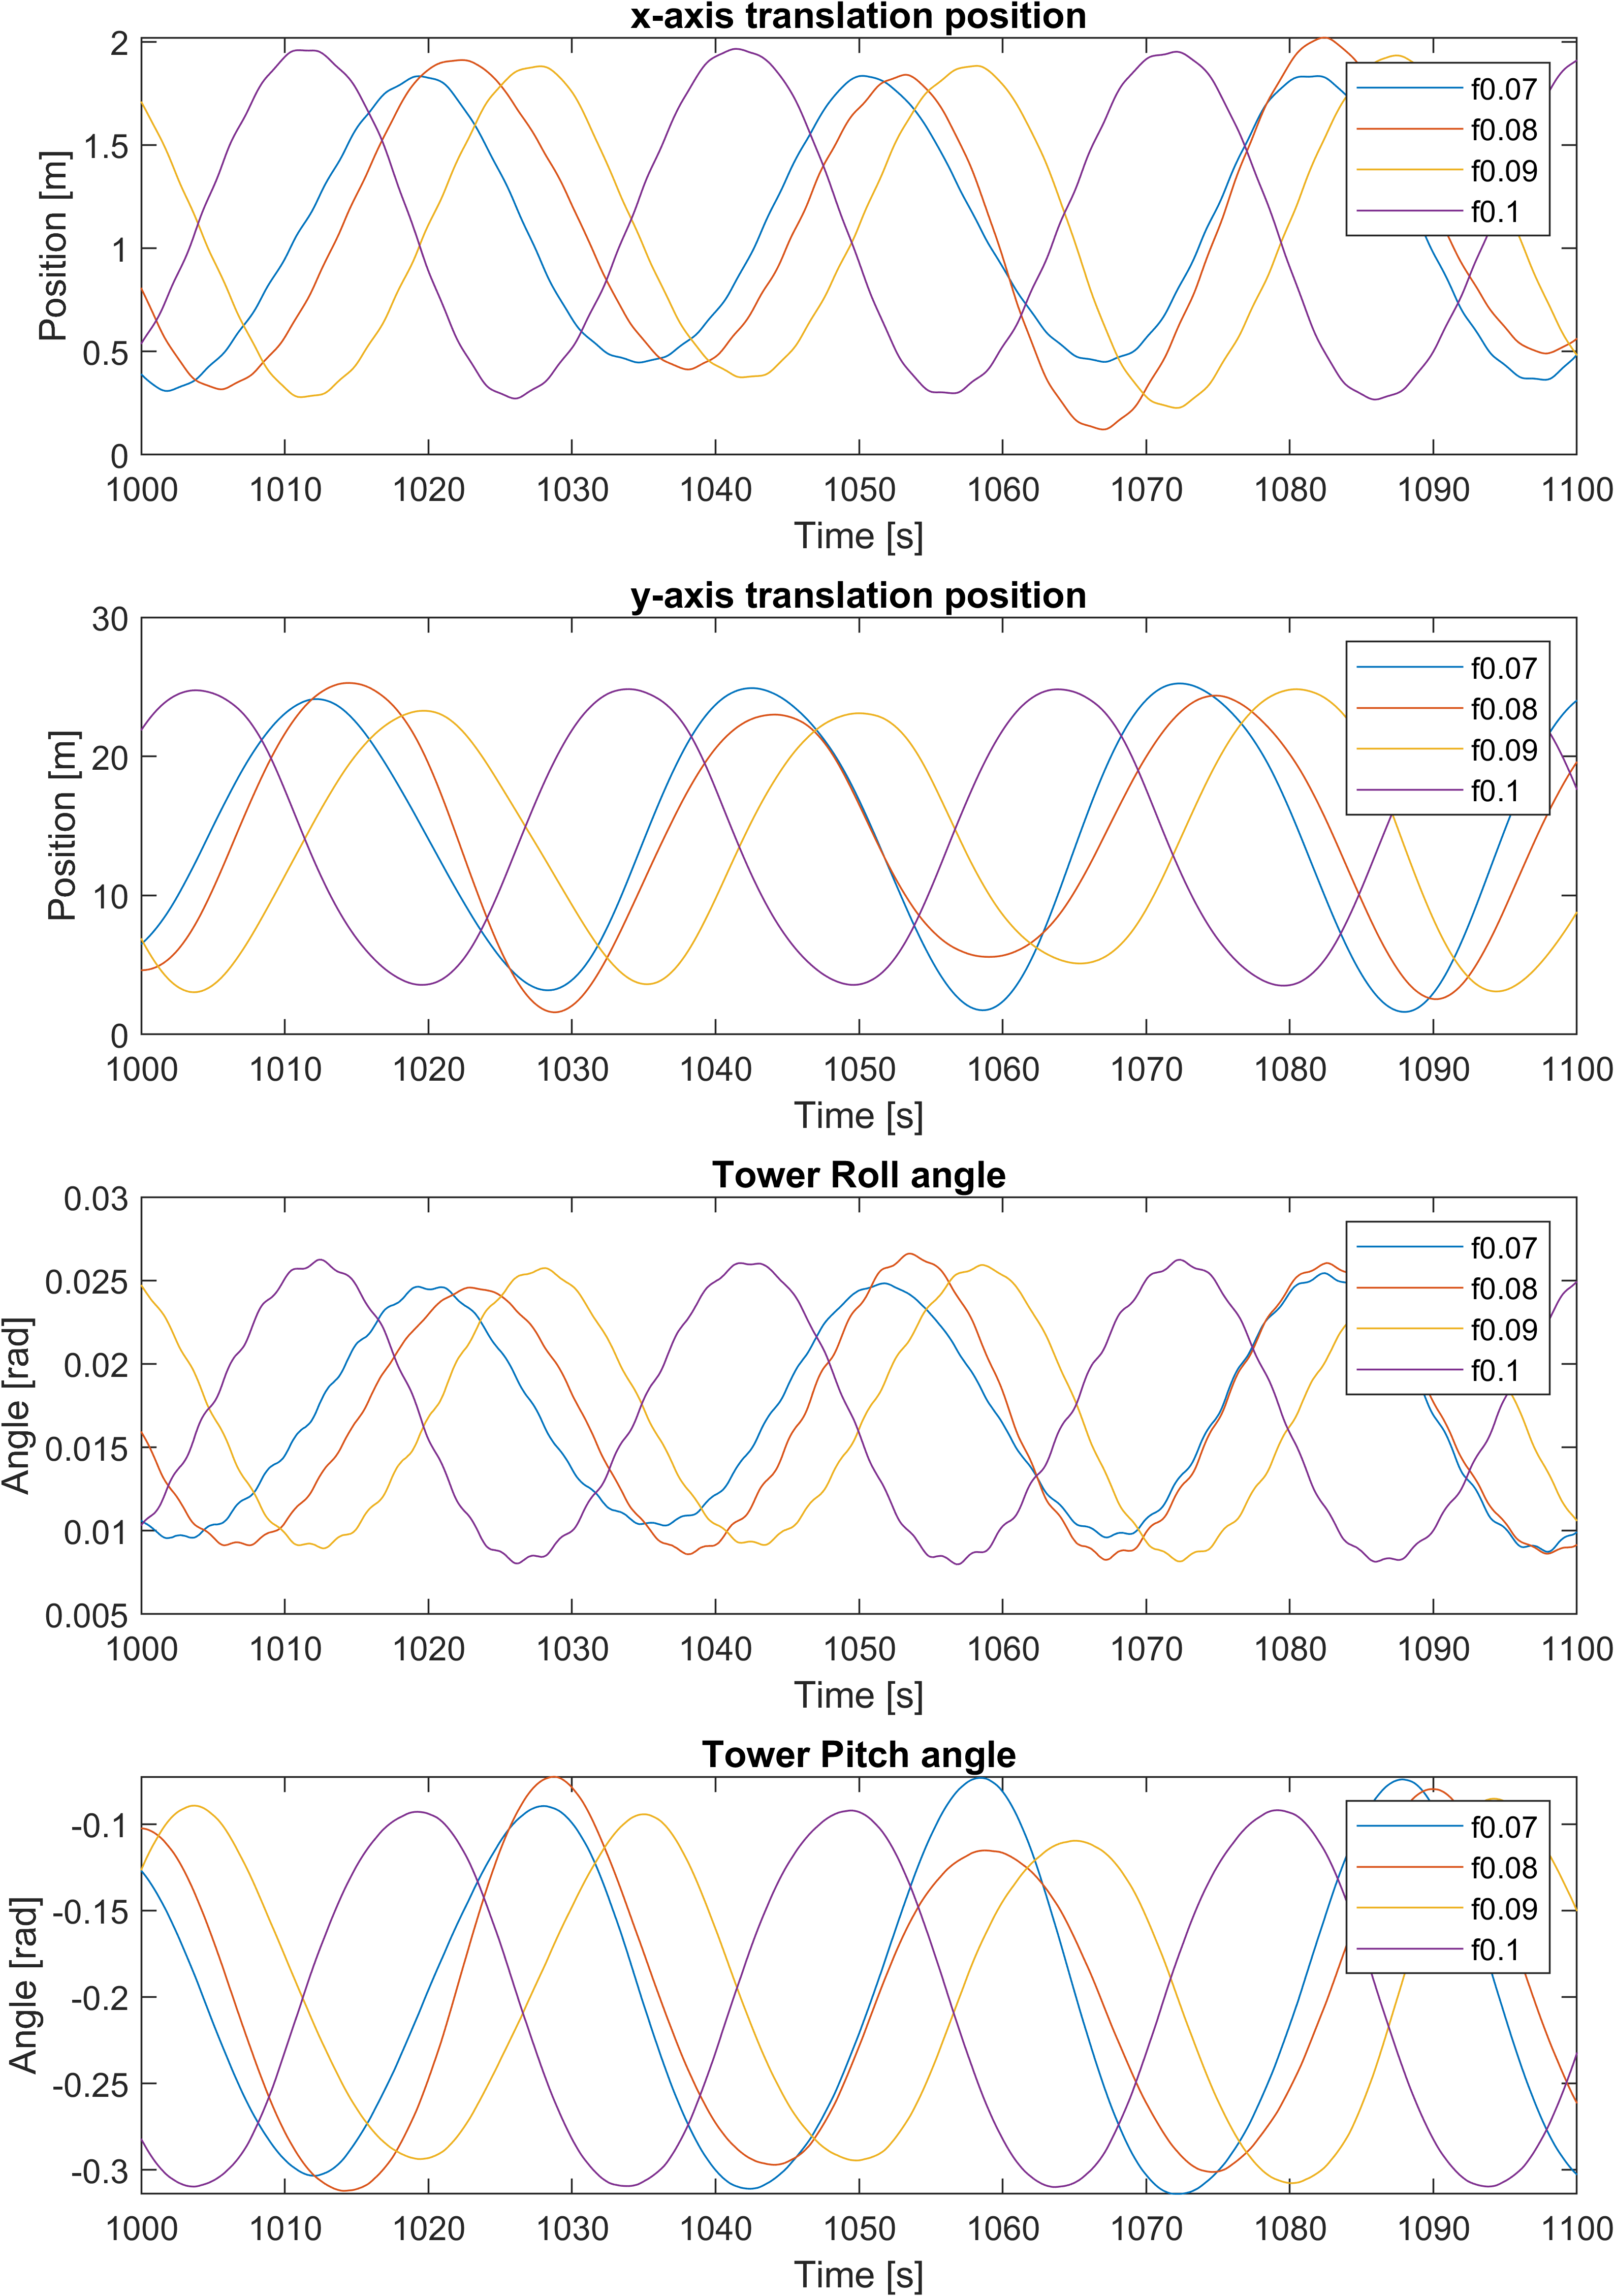
\includegraphics[width=0.8\linewidth]{Graphics/TestResults/tj00/tjj0_f07to1_xPosToPitchAng.png}
	\caption{Plot of x- and y-axis translation position and tower roll and pitch angle for the injected rotor angular velocity frequencies 0.07 Hz, 0.08 Hz, 0.09 Hz and 0.1 Hz. The natural frequency of the turbine in the water is apparent in both the translation and pitch.}
	\label{fig:tjj0_f07to1_xPosToPitchAng}
\end{figure}

\begin{figure}[h]
	\centering
	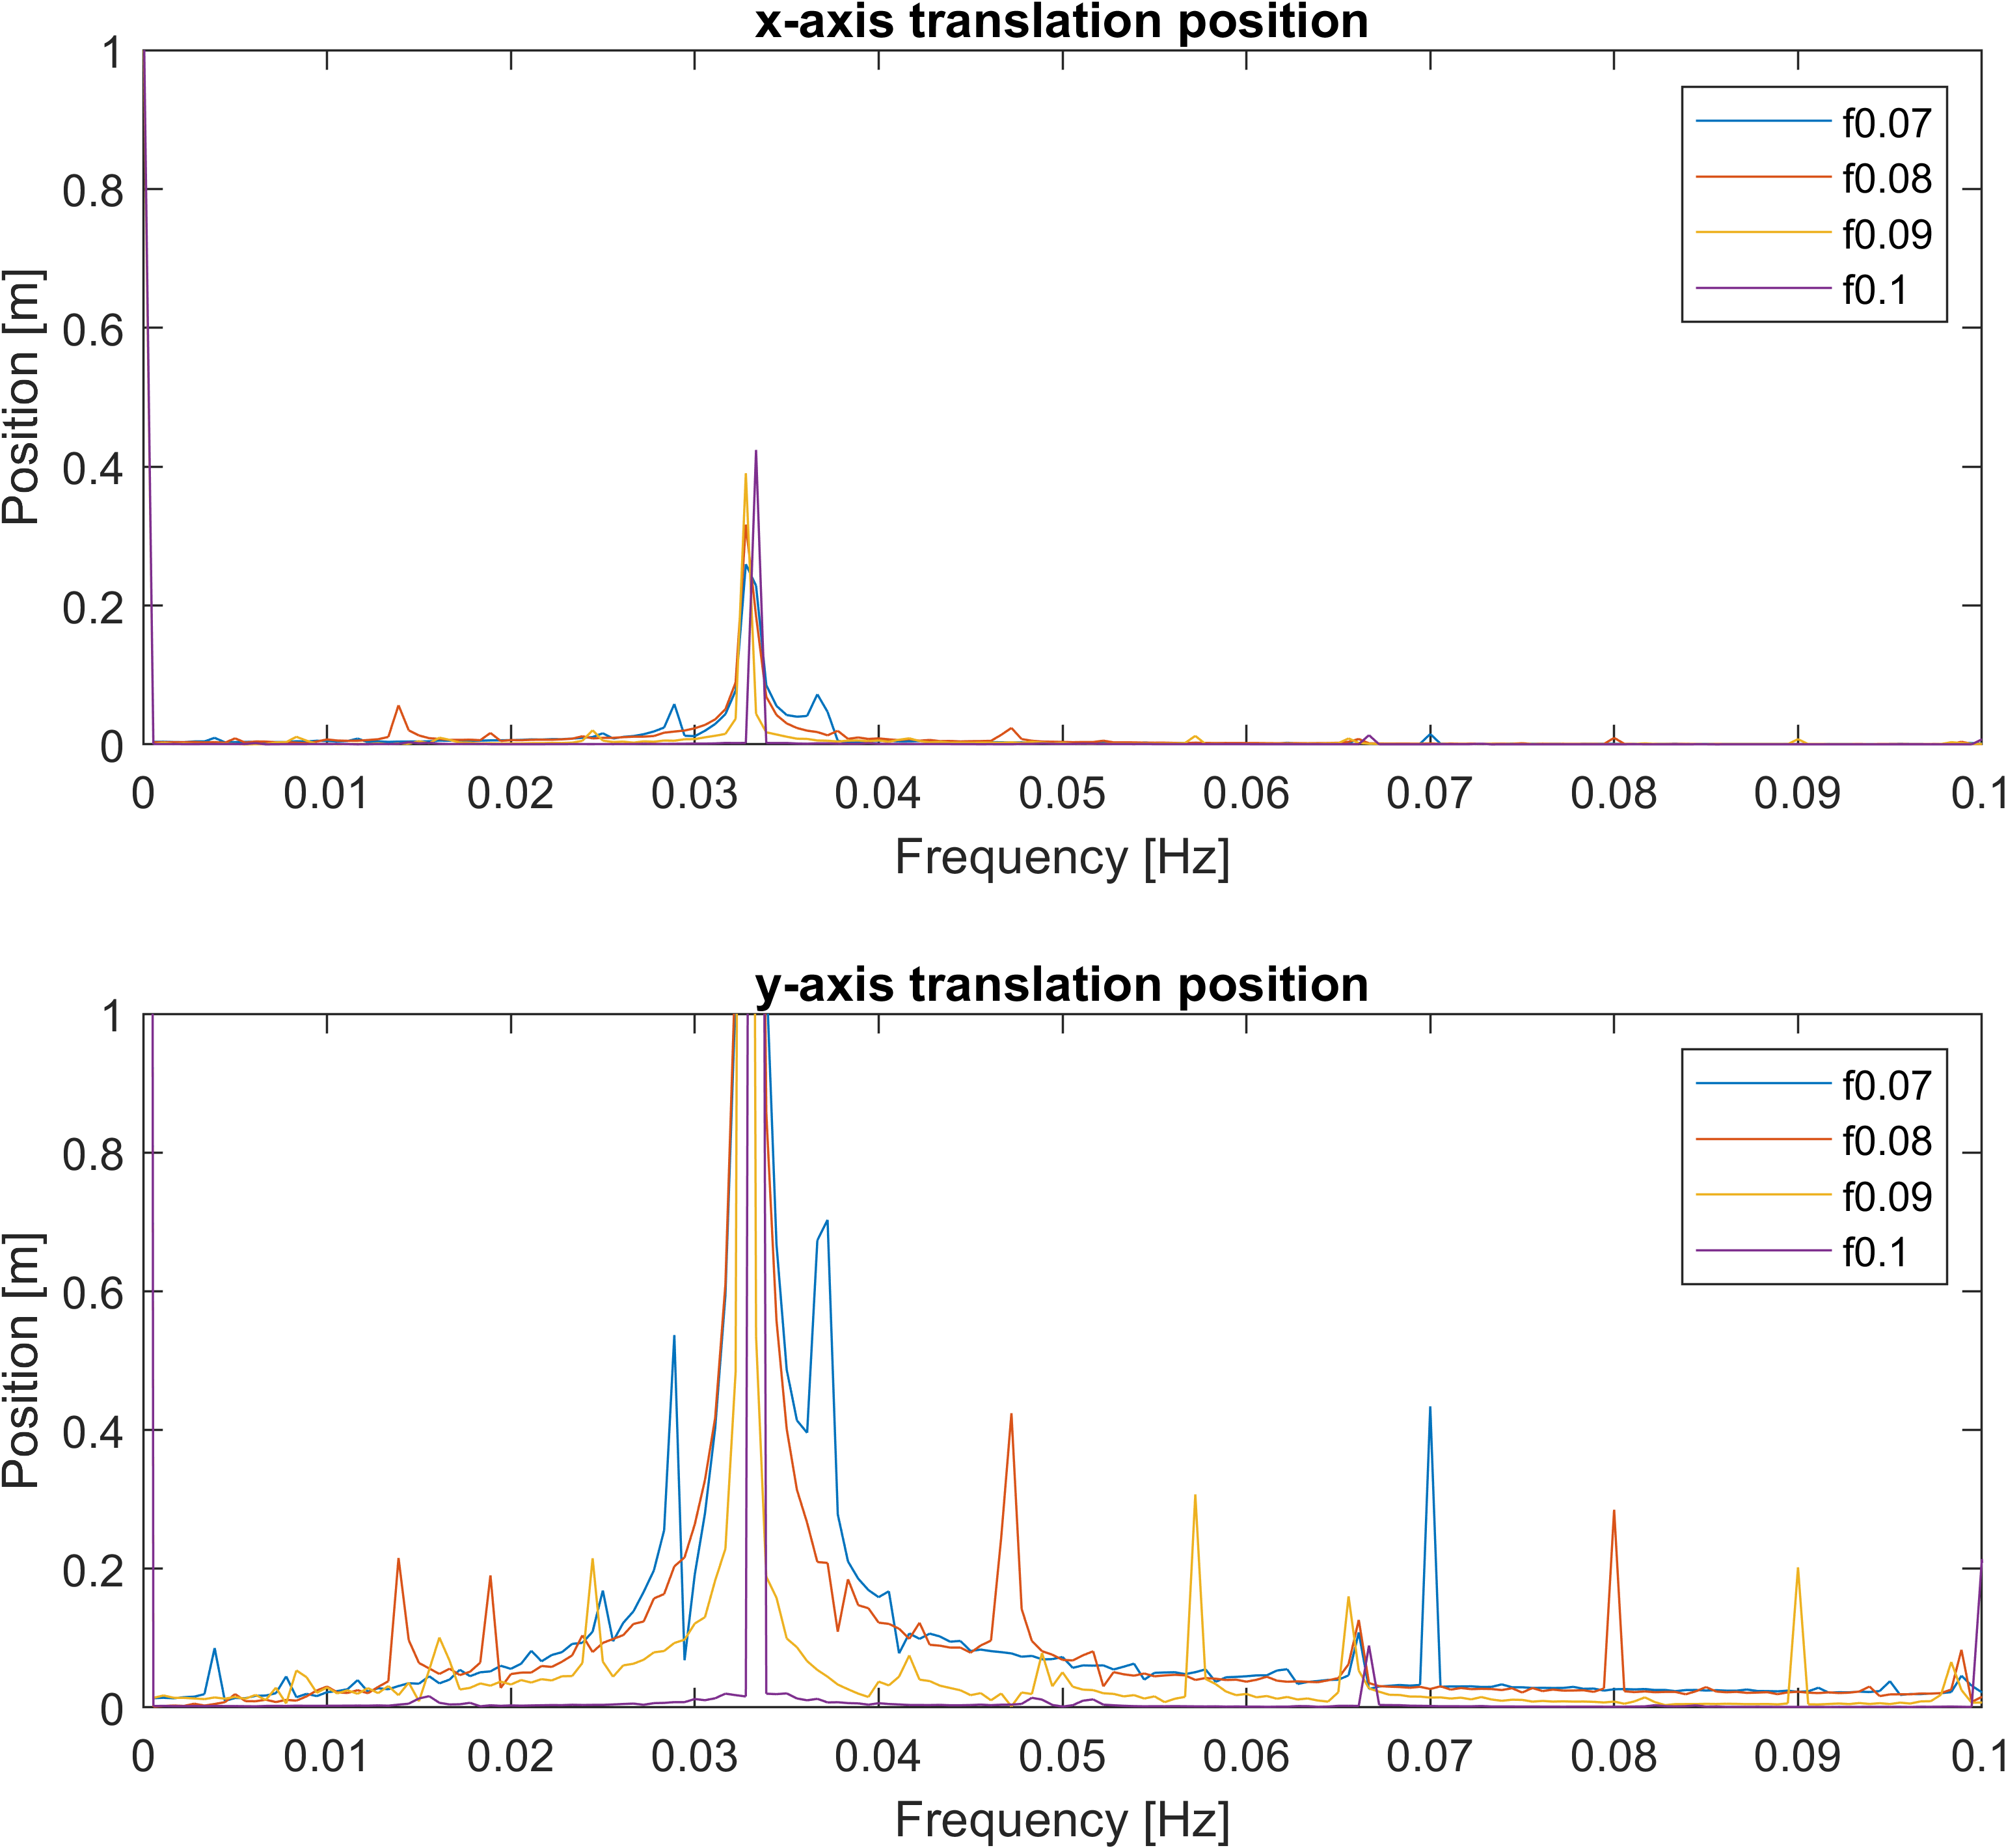
\includegraphics[width=0.8\linewidth]{Graphics/TestResults/tj00/tjj0_f07to1_xPosyPosFFT.png}
	\caption{Plot of FFT of x- and y-axis translation position for the injected rotor angular velocity frequencies 0.07 Hz, 0.08 Hz, 0.09 Hz and 0.1 Hz. The natural frequency of the turbine is greatly apparent around 0.034 Hz especially in the y-translation position subplot. The injected frequencies are visible at their respective frequencies, especially for the y-axis translation position. It is also visible that lower frequencies are translated better.}
	\label{fig:tjj0_f07to1_xPosyPosFFT}
\end{figure}

\begin{figure}[h]
	\centering
	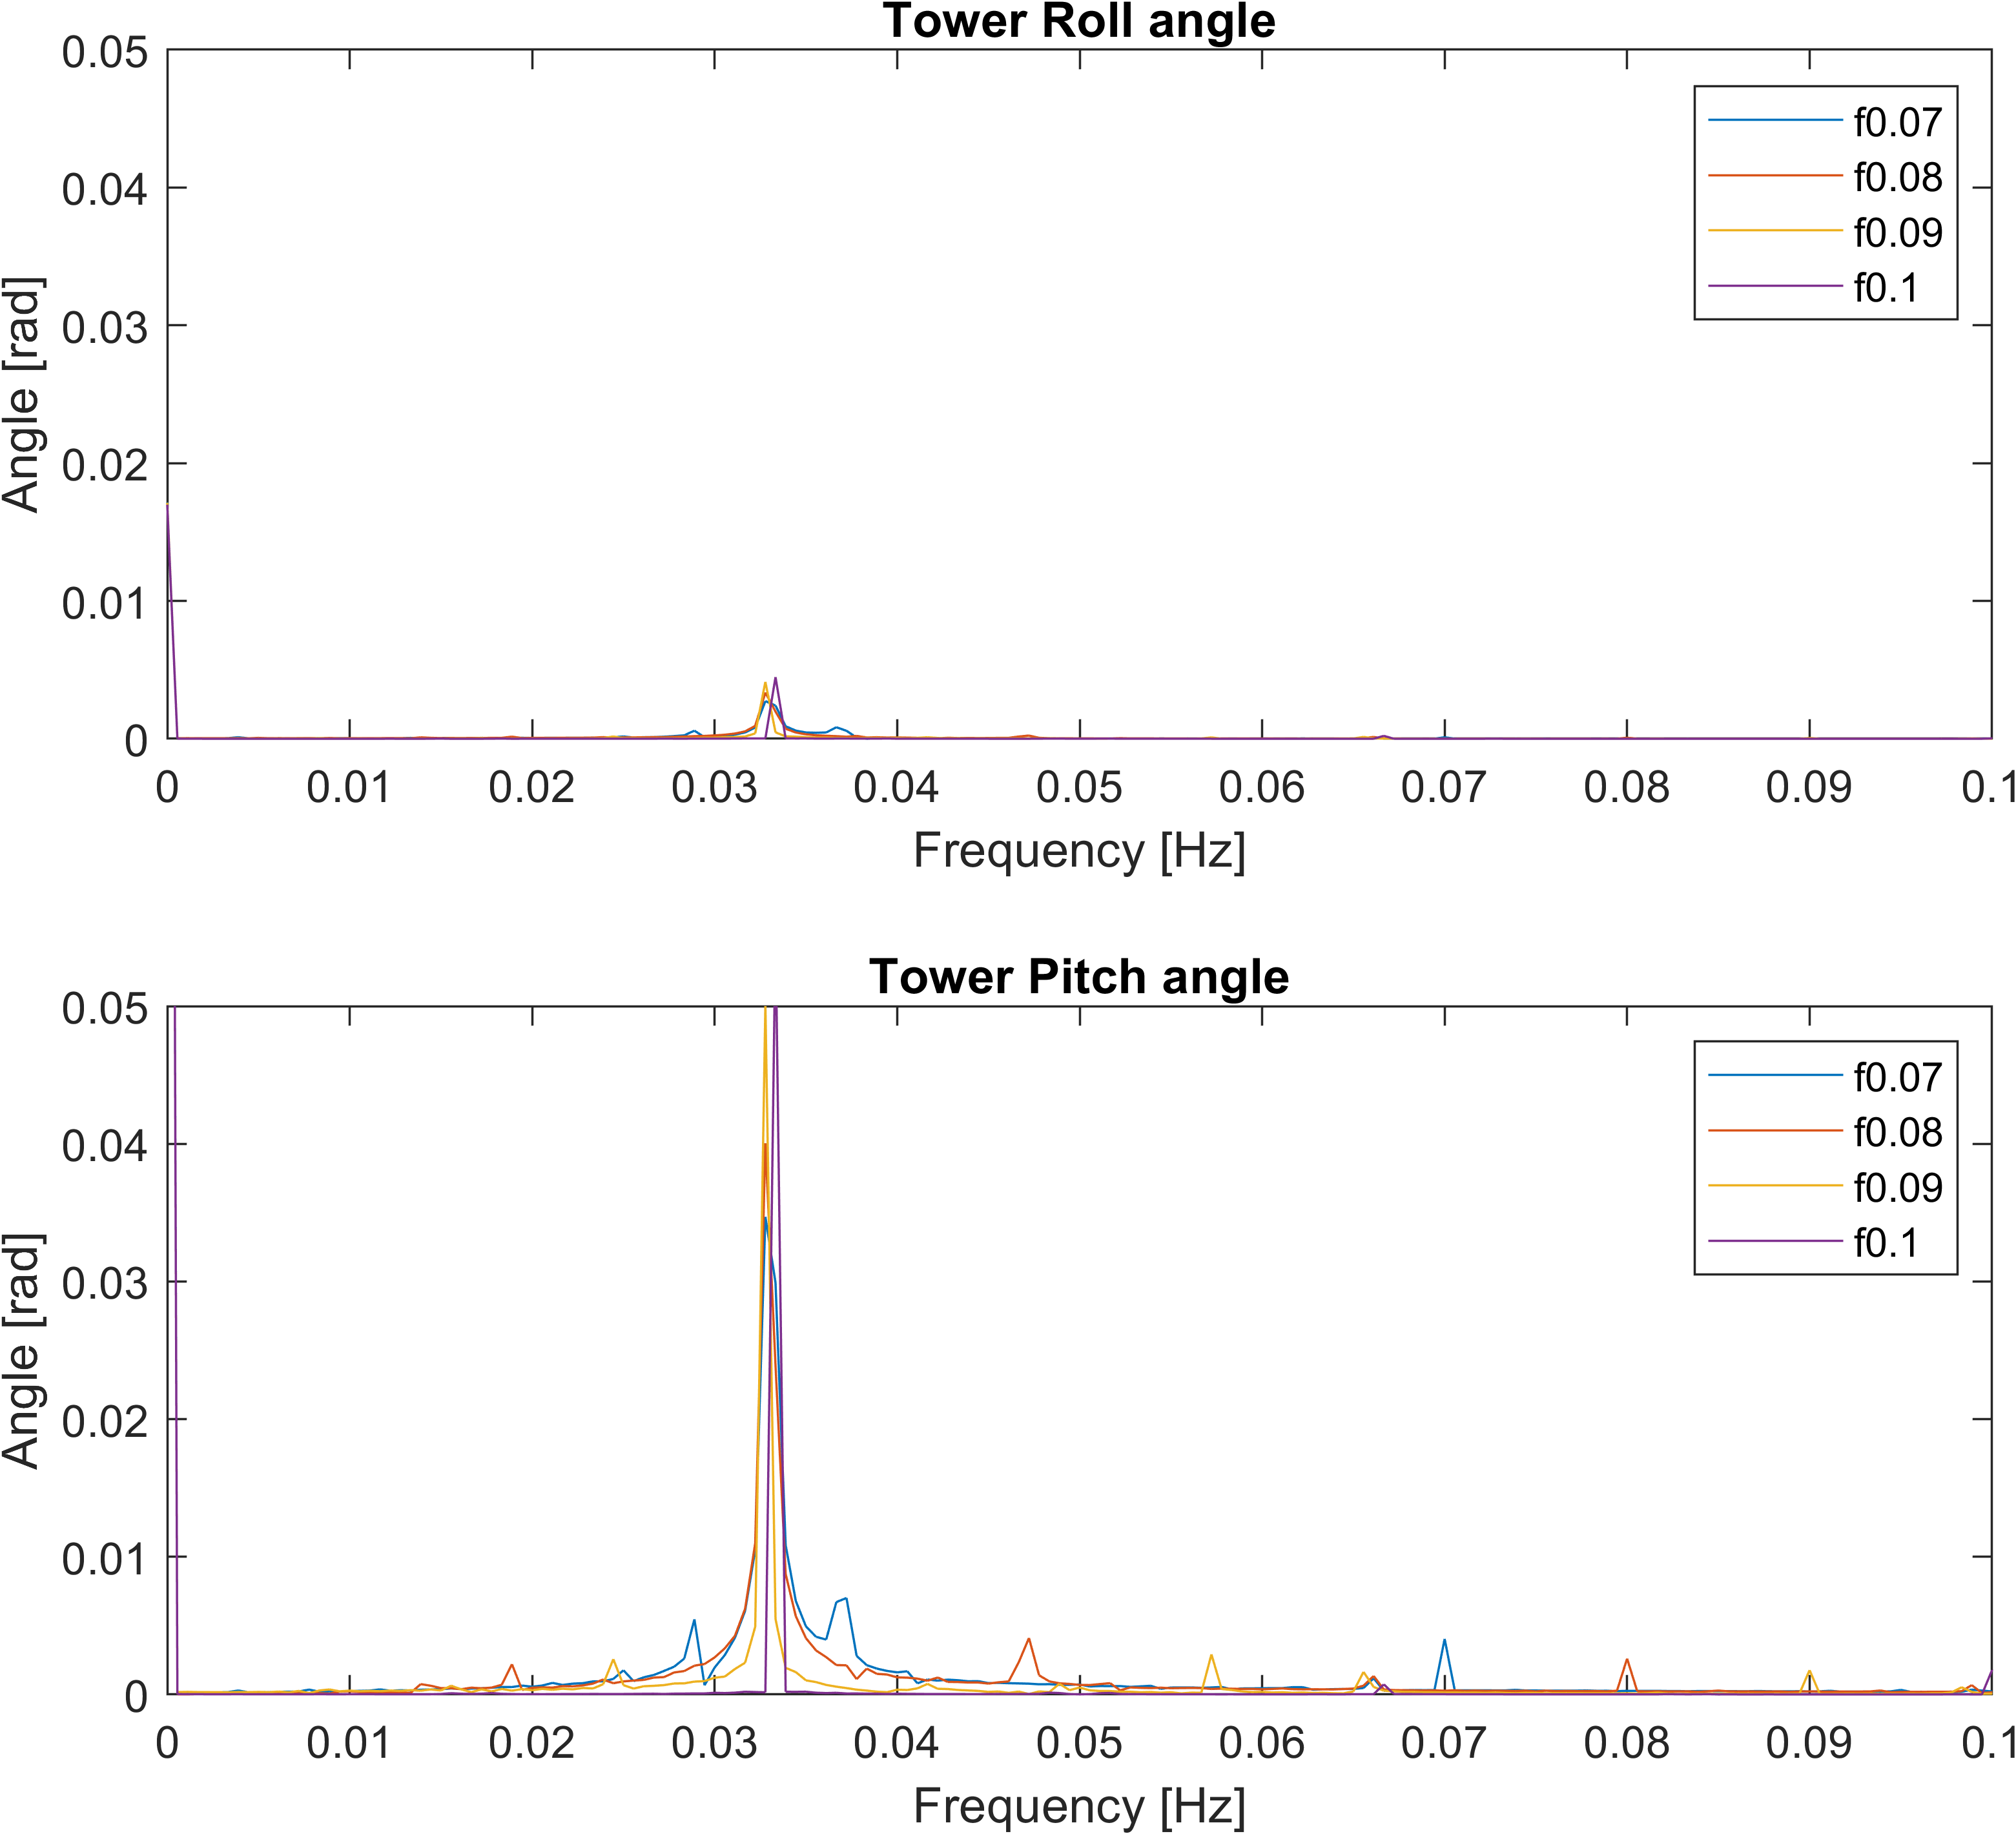
\includegraphics[width=0.8\linewidth]{Graphics/TestResults/tj00/tjj0_f07to1_RollPitchAngFFT.png}
	\caption{Plot of FFT of roll and pitch angle for the injected rotor angular velocity frequencies 0.07 Hz, 0.08 Hz, 0.09 Hz and 0.1 Hz. The natural frequency of the turbine is greatly apparent around 0.034 Hz especially in the pitch angle. The injected frequencies are visible at their respective frequencies, especially for the pitch angle. It is also visible that lower frequencies are translated better.}
	\label{fig:tjj0_f07to1_RollPitchAngFFT}
\end{figure}

%\begin{figure}[h]
%	\centering
%	\includegraphics[width=0.8\linewidth]{Graphics/TestResults/tj00/}
%	\caption{}
%	\label{fig:tj00_}
%\end{figure}
%
%\begin{figure}[h]
%	\centering
%	\includegraphics[width=0.8\linewidth]{Graphics/TestResults/tj00/}
%	\caption{}
%	\label{fig:tj00_}
%\end{figure}


\subsubsection{Sources of error and insecurities}
